\section{Looking for Underlying Structure}
\label{sec:PCA}
The size of our testing set is 8965 $\times$ 397. However, we suspect that at least some of these data points are redundant. This section will explore some of the underlying structure of the data by looking at correlations between variables and employing dimension reduction techniques such as principal component analysis (PCA) and independent component analysis (IPA). 
\subsection{Correlations}
The first line of attack is to calculate the correlation matrix. It will provide two pieces of information. First, presence of large non-zero off-diagonal values in this matrix will be a good indication that redundant dimensions are present. Second, correlations of our response variable C1 with other variables might indicate which variables are tied most closely together with binge drinking. We applied cor() to the data, and sorted the results by column C1, which we earlier picked as the response variable. The top twenty variables are given in Tab.\ref{correlations}. These results are disappointing in the sense that we did not learn anything new about the data, merely discovered a lot of redundancy. 

\begin{center}
\begin{table*}[ht]
\begin{tabular}{l l l}
\hline \hline
Correlation with C1 & Variable Name &Short summary of the variable given in the Codebook\\ \hline 
0.900 & FREQBING	&Frequent binger\\
0.837 & DRINKCAT	&Levels of drinking and binging\\
0.773 & BINGE		&Students binge in college\\
0.742 & VOL30		&Average number of drinks last 30 days\\
0.666 & NUMPROB	&Problems with alcohol\\
0.648 & C7		&Current use of alcohol\\
0.633 & C2		&Past 2 weeks - four drinks in a row\\
0.606 & PERSIST	&Continue high school drinking behavior\\
0.598 & D4A		&Compare own drinking to other students\\
-0.579 & NOBINGE	&Never a binger\\
\hline
\end{tabular}
\caption{Top 10 correlations with C1. Evidently, drinking is related to drinking. These data suggest that dimension reduction could be useful to get rid of redundant data and make the important relationships between alcohol and other variables clearer.}
\label{correlations}
\end{table*}
\end{center}

Redundancy in the data can be addressed by applying dimension reduction using principal component analysis.
\subsection{Principal Component Analysis}
In this subsection, we used the standard R function prcomp() to reduce the number of variables from 397 to 4 by singular value decomposition (SVD) \cite{berrar}. A brief summary of SVD follows. 

We define left- and right-singular vectors, $u$ and $v$, such that:

\begin{equation}
Xv=su,~X^*u = sv;
\end{equation}
where each $s$ is a singular value of $X$. We are interested in finding these vectors because it can be shown that a least-squares approximation to $X$ equals $\sum_{k=1}^{l}u_ks_kv_k^T$. In order to take advantage of this property to analyze a $m\times n$ matrix $X$ containing $m$ observations of $n$ variables, we look for solve $X = USV^T$. Here $U$ contains a set of left singular vectors $u_k$, and $V$ contains the set of right singular vectors $v_k$, and $S$ is a diagonal matrix containing singular values $s_k$, where $k = 1, ..., n$. 

%
%\begin{figure}
%\centering
%%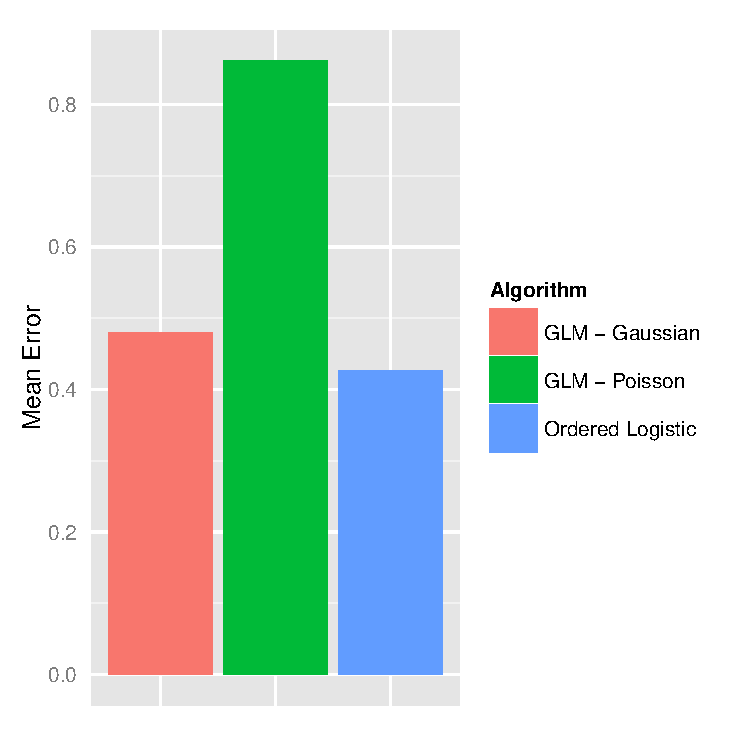
\includegraphics[scale=0.5]{linear_plus_pca.pdf}
%\caption{Mean error using three kinds of regression on a dataset whose dimension has been reduced by PCA.}
%\label{}
%\end{figure}


\begin{center}
\begin{table*}[ht]
\begin{tabular}{l l l l}
\hline \hline
Component 1 & Component 2 &Component 3&Component 4\\ \hline 
\hline
\end{tabular}
\caption{Top five terms in each component.}
\label{components}
\end{table*}
\end{center}

Let us see how dimension-reduced analysis will compare to previous methods. As usual, we are performing a five-fold validation procedure. We run PCA on the training set to extract four principal components, and their mixing coefficients for each observation. We then fit the response variable to these four dimensions using several regression algorithms. Finally, we calculate the mixing coefficients using the same principal components, but in the testing set, and use them to predict C1. 

The predictive error using three different regression algorithms after PCA are plotted in Fig. \ref{linear_plus_pca}. The lowest error we have obtained is 0.42, which is very close to the best error from applying regression on all 397 variables. 

\begin{figure}
\centering
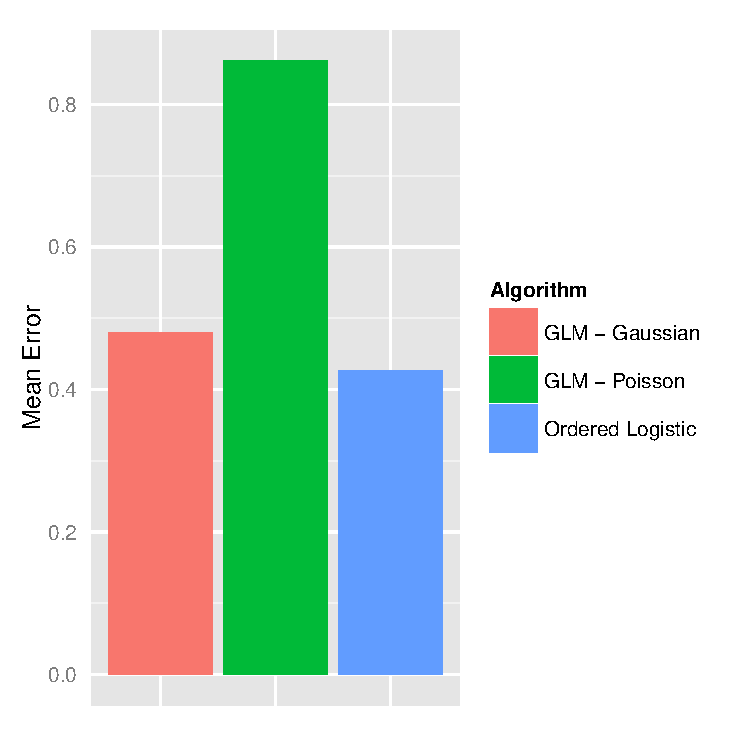
\includegraphics[scale=0.5]{linear_plus_pca.pdf}
\caption{Mean error using three kinds of regression on a dataset whose dimension has been reduced by PCA.}
\label{linear_plus_pca}
\end{figure}

The most amazing thing about PCA is that in the end, four numbers were sufficient to encode 397 variables without losing any noticeable accuracy of prediction.